\documentclass[main.tex]{subfiles}
\begin{document}
\author{Philipp Nickel}
\section{Der Datensatz CTU13}
\subsection{Herkunft}
Der CTU-13 ist ein Datensatz aus Botnet Traffic, welcher von der Czech Technical University in Prag, im Jahr 2011 aufgezeichnet wurde. 
\subsection{Struktur}
Das Ziel der Aufzeichnung war es, einen großen Datensatz von realem Botnet Traffic vermischt mit Normal und Background Traffic zu erstellen. Insgesamt besteht der Datensatz aus 13 Aufzeichnungen (weiterführend als Szenarios bezeichnet). In jedem Szenario wurden verschiedene, spezifische Arten von Malware ausgeführt. Dabei wurden unterschiedliche Protokolle genutzt und verschiedene Aktionen ausgeführt. \ \\

In der folgenden Tabelle ist festgehalten, in welchen Szenarien welche Malware aufgetreten ist. Dabei kann es sich um die Nutzung von IRC, P2P und HTTP Protokollen sowie das Versenden von SPAM oder das Betreiben von Click-Fraud oder DDos-Angriffen handeln. Außerdem können Ports gescannt, Fast-Flux Techniken angewandt oder Custom Compiling betrieben worden sein. \\
\begin{figure}[ht]
 \centering
 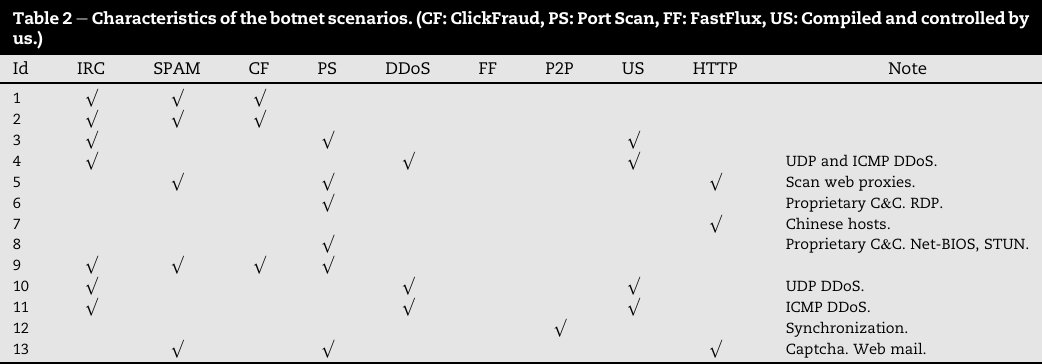
\includegraphics[width=1\textwidth]{images/CTU_Tabelle_1.jpg}
 \caption{Charakteristika der Szenarien}
 \label{Tabelle Charakteristika der Szenarien}
\end{figure}

 % Quelle http://mcfp.weebly.com/the-ctu-13-dataset-a-labeled-dataset-with-botnet-normal-and-background-traffic.html


In der folgenden Tabelle die Aufzeichnungsdauer der einzelnen Szenarien, die Anzahl der Packete, die Anzahl an Netflow und die Größe der pcap-Datei eingesehen werden. Zusätzlich enthält die Tabelle die in den Szenarios benutzte Malware und die Anzahl an infizierten Rechnern.

% Quelle http://mcfp.weebly.com/the-ctu-13-dataset-a-labeled-dataset-with-botnet-normal-and-background-traffic.html

\begin{figure}[ht]
 \centering
 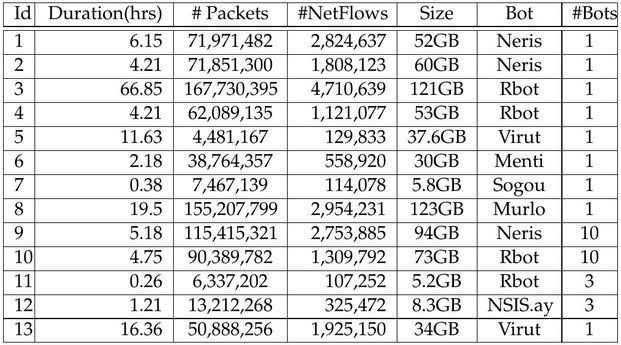
\includegraphics[width=1\textwidth]{images/CTU_Tabelle_2.jpg}
 \caption{Daten für jedes Szenario}
 \label{Daten für jedes Szenario}
\end{figure}

Die finale NetFlow-Datei besteht aus den folgenden Feldern:
\begin{center}
\begin{enumerate}
\item Start Time
\item End Time
\item Duration
\item Source IP address
\item Source Port
\item Direction
\item Destination IP address
\item Destination Port
\item State
\item SToS
\item Total Packets
\item Total Bytes
\end{enumerate}
\end{center}
Insgesamt umfasst der CTU-13 Datensatz bis zu 662.9 GB an pcap-Dateien.  \\
\subsection{Besonderheiten}
Der CTU13-Datensatz enthält im Vergleich zu anderen Datensätzen einige Besonderheiten. Diese Besonderheiten werden im Verlauf dieses Kapitels genauer erläutert.
\subsubsection{Label}
% Besonderheit der Labels: Botnet, background, normal
Während der Erstellung des Datensatzes wurden 3 verschiedene Labels vergeben: Background, Botnet und Normal. Diese wurden nach folgender Priorität vergeben: 
\begin{center}
\begin{enumerate}
\item Dem gesamten Traffic das Background Label zuordnen,
\item Das Normal Label dem Traffic zuordnen, der bestimmten Filtern entspricht,
\item Jedem Traffic das Label Botnet zuordnen, der von oder zu einer bekannten infizierten IP Adresse kommt.
\end{enumerate}
\end{center}
Die genutzten Filter wurden von bekannten und kontrollierten Computern im Netzwerk, wie Routern, Proxies, Switches und eigenen Laborrechnern erstellt.
\subsubsection{Bidirectional Netflow}
 Der in dem Projekt genutzte CTU-13 Datensatz enthält bidirectional NetFlows. Diese bidirectional NetFlows haben gegenüber directional NetFlows folgende Vorteile: 
\begin{center}
\begin{enumerate}
\item Das Problem der Differenzierung zwischen Client und Server wird damit gelöst.
\item Sie enthalten mehr Informationen.
\item Sie enthalten detailliertere Labels.
\end{enumerate}
\end{center}
\subsubsection{Manuell gelabelt}
Die Szenarios des CTU-13 Datensatzes wurden manuell analysiert und gelabelt. Der Prozess der Labelverteilung erfolgte innerhalb der NetFlow Dateien.
\subsubsection{NetFlow}
Zur weiteren Verwendung und Analyse des CTU-13 Datensatzes stehen die kompletten pcap-Dateien aus Datenschutzgründen nicht zur Verfügung.
%\subsection{Entscheidung}

\end{document}


